\documentclass[10pt,letterpaper]{article}

% Content-reconstruction draft for an AAAI submission. The official AAAI
% style file is intentionally not vendored here; replace this compact draft
% preamble with the current AAAI author-kit preamble before submission.
\usepackage[T1]{fontenc}
\usepackage{times}
\usepackage{amsmath,amssymb,amsthm}
\usepackage{booktabs}
\usepackage{graphicx}
\graphicspath{{../figures/}}
\usepackage{float}
\usepackage{xcolor}
\usepackage{url}
\usepackage{microtype}
\usepackage[margin=0.9in]{geometry}
\usepackage[numbers]{natbib}
\usepackage{hyperref}
\hypersetup{hidelinks}
\urlstyle{same}

\newcommand{\lifeline}{\textsc{Lifeline}}
\newcommand{\method}{\textsc{Topology-GNN}}
\newtheorem{definition}{Definition}
\newtheorem{proposition}{Proposition}

\title{LIFELINE: An Auditable Rule--State Benchmark for Self-Play}
\author{Anonymous Authors}
\date{}

\begin{document}
\maketitle

\begin{abstract}
We introduce LIFELINE, a deterministic self-play benchmark designed to expose
confounding between physical occupancy, player-specific logical connectivity,
cascading removal, repetition history, and legal-action masks. The benchmark
provides exact snapshots, replayable trajectories, and explicit observation
projections for rule and state audits. Complete side-five enumeration finds
reachable latent topology differences but no difference in legal actions,
transitions, exact values, or optimal actions. A standard-start side-six
paired-history witness reaches the same deliberately mask-free topology while
Superko changes the legality of one shared placement; the implemented masks
still differ, so the witness is not an implemented-observation alias.

We also report a receipt-bound audit of padded-CNN, physical-edge Grid-GNN, and
typed-edge Topology-GNN baselines on jointly trained sizes 5, 7, and 9. All
45 final seed scores against Random exceed 0.5, while direct-play summaries
against UCT-MCTS-16 are heterogeneous and each evaluation task repeats only
two deterministic trajectories. These results are descriptive and do not
support a global representation ranking, a learned feature benefit, or
unseen-size generalization. LIFELINE is therefore presented as an auditable
benchmark and diagnostic resource, with stronger causal and cross-game claims
left for future experiments.
\end{abstract}

\section{Introduction}
\label{sec:introduction}

Board-game agents are often evaluated as if the visible board were the whole
state. That assumption becomes difficult to audit when rules maintain hidden
connectivity, cascade removals, or repetition history, and when the learning
interface also exposes an invalid-action mask. A benchmark can then report a
representation difference without showing whether the difference is caused by
the intended structural input, by legality information, or by an evaluation
artifact.

LIFELINE is designed to make these distinctions explicit. Its triangular
lattice separates rendered occupancy from player-specific logical
connectivity; attacks can cut edges and remove disconnected components; and a
Superko rule makes legality depend on the complete history. We use the game as
a controlled audit setting rather than as evidence that one neural
representation is universally better. The questions are: (1) which state
components can be separated and replayed exactly, (2) when does a weaker
observation projection hide a legality difference, and (3) what can a small,
receipt-bound self-play comparison actually establish?

Our contributions, each tied to an auditable artifact and an explicit boundary,
are:
\begin{enumerate}
  \item an auditable, variable-size self-play environment with exact
  snapshots, legal masks, replayable trajectories, and recorded rule-engine
  parity traces;
  \item a diagnostic protocol that separates latent topology differences from
  decision-relevant legality, including an exhaustive side-five negative
  result and a bounded side-six mask-free history witness; and
  \item a frozen five-seed baseline audit backed by 330 receipts and 30,600
  task-indexed replay-verified game records, together with explicit limits on
  what the comparison can say about representations.
\end{enumerate}

The benchmark contribution does not depend on a positive model result. We do
not claim that topology or compact history improves learning, that the
implemented Grid observation is non-Markov, that any representation is
globally superior, or that the results generalize to unseen sizes or other
games without corresponding formal evidence.

\paragraph{Claim control.}
A frozen claim--evidence--limitation ledger accompanies the draft. Every primary
claim names its authoritative CSV/JSON or verifier and retains the relevant
scope restriction; failed and inconclusive cells remain in all tables.

\section{Related Work}
\label{sec:related}

\paragraph{Self-play and game environments.}
AlphaGo Zero and AlphaZero established policy--value learning with search from
self-play, while expert iteration, ELF OpenGo, and MuZero broadened the
algorithmic and reproducibility picture
\citep{silver2017mastering,silver2018general,anthony2017thinking,
tian2019elf,schrittwieser2020mastering}. General-purpose multi-agent and game
testbeds include OpenSpiel and PettingZoo
\citep{lanctot2019openspiel,terry2020pettingzoo}; PGX supplies
hardware-accelerated parallel game simulators for reinforcement learning
\citep{koyamada2023pgx}. MCTS is surveyed by \citet{browne2012survey}.
\lifeline{} is narrower than these platforms but
targets a particular confound: rendered occupancy, player-specific logical
connectivity, and repetition history can be distinct parts of simulator state.

\paragraph{General game systems and structural transfer.}
Ludii and Regular Boardgames provide complementary declarative systems for
representing and executing board-game rules, including dedicated reasoning
work for the latter \citep{piette2020ludii,kowalski2019regular,
kowalski2020efficient}; Polygames supplies zero-learning infrastructure across
multiple games \citep{cazenave2021polygames}. Prior work transfers
policy--value networks across Hex sizes, games, and variants
\citep{gao2019transferable,soemers2021transfer}; AlphaZero with GNNs has also
been studied for scaling from small to larger board games
\citep{benassayag2021smalllarge}. Graph representations are evaluated directly
in chess RL and DQN-based Hex agents
\citep{rigaux2024chessgraph,keller2023hexgnn}. These studies are the closest
empirical neighbors, but do not establish topology-input superiority in
\lifeline{} or unseen-size transfer for our models.

\paragraph{Graph representations and size.}
Message passing, inductive graph learning, relational biases, and graph
reinforcement learning motivate explicit structural inputs
\citep{gilmer2017neural,hamilton2017inductive,battaglia2018relational,
jiang2018graph}. Work on neural algorithm execution, combinatorial
optimization, and TSP generalization shows why graph structure alone does not
justify extrapolation claims \citep{xu2019what,joshi2020learning}. We therefore compare representations only
on jointly trained sizes and reserve unseen-size evaluation for future formal
artifacts.

\paragraph{State sufficiency, masks, and repetition.}
Partial observability, perceptual aliasing, and state abstraction formalize the
risks of discarding history or decision-relevant variables
\citep{kaelbling1998planning,chrisman1992perceptual,
givan2003equivalence,abel2017near}. Invalid-action masking further shows that
legality information is part of the learning interface
\citep{huang2022invalid}. Graph-history interaction is an established
rules/search issue \citep{campbell1985graphhistory,kishimoto2004graph},
including in Chinese chess \citep{wu2006graphhistory}. Go's legality,
combinatorics, and legal-position counting provide closely related precedent
for repetition-sensitive state accounting
\citep{tromp2007combinatorics,tromp2016number}. Our
diagnostics accordingly distinguish a full simulator
state, an implemented masked observation, and deliberately weaker projections.

\section{The LIFELINE Benchmark}
\label{sec:environment}

\subsection{Board and actions}

A board of side length $n$ contains
\begin{equation}
  N(n) = \frac{n(n+1)}{2}
\end{equation}
valid lattice points. A turn selects one lattice point or the pass action, for
$N(n)+1$ discrete actions. The main benchmark uses two players and canonicalizes
the observation to the player to act.

\subsection{Physical occupancy and logical topology}

Let $B_t$ denote physical point occupancy and let
$E_t^{(b)}, E_t^{(w)}$ denote the explicit logical edge sets of the two players.
Physical line points are used for rendering and blocking, whereas logical edges
define connectivity to the protected initial node. An attack can break an edge
and remove nodes and line points that are no longer logically connected.

\begin{figure}[t]
  \centering
  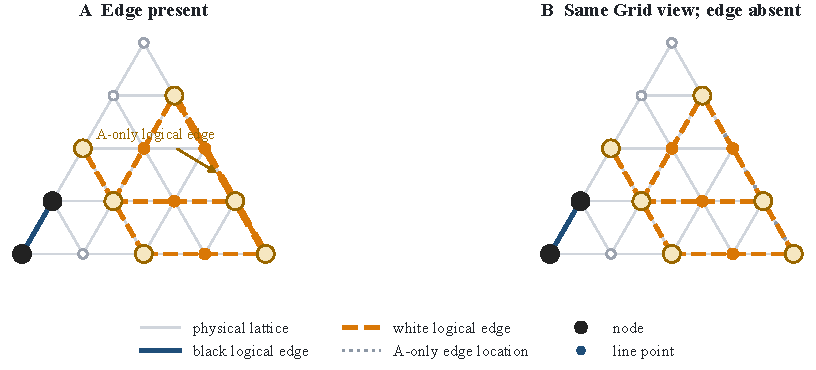
\includegraphics[width=0.94\linewidth]{fig1_lifeline_logical_edges.pdf}
  \caption{A replay-verified state pair reconstructed from the frozen side-five
  witness ledger. Both reachable states have identical
  occupancy, player to act, pass count, and legal mask; only history A contains
  the highlighted white logical edge. The dotted segment in history B marks
  that edge's absent location. This demonstrates latent topology aliasing only:
  the exhaustive side-five audit found no decision-relevant consequence.}
  \label{fig:logical-edges}
\end{figure}

\subsection{Full simulator state}

We model the full state as
\begin{equation}
  x_t = \left(B_t, E_t^{(b)}, E_t^{(w)}, H_t, p_t, c_t, z_t\right),
\end{equation}
where $H_t$ is the visited-state set used by the repetition rule, $p_t$ is the
player to act, $c_t$ is the consecutive-pass count, and $z_t$ is the terminal
flag and cached terminal outcome. Resignation is outside the frozen training
environment.

\subsection{Observation protocols}

\begin{table}[t]
  \centering
  \caption{Pre-registered observation variants from the frozen benchmark
  protocol. The simulator always retains the exact full state; the table does
  not imply that any exposed feature is independently necessary.}
  \label{tab:observations}
  \begin{tabular}{lll}
    \toprule
    Name & Exposed structure & Purpose \\
    \midrule
    Grid & Occupancy and turn features & Flat/spatial baseline \\
    GridGraph & Grid plus fixed lattice edges & Size-agnostic graph baseline \\
    Topology & GridGraph plus typed logical edges & Topology-input baseline \\
    TopologyHistory & Topology plus compact history features & Planned history ablation \\
    \bottomrule
  \end{tabular}
\end{table}

All four protocols also expose the player to act, consecutive-pass count, and
legal-action mask. Thus a legal-set difference alone is not an alias under the
implemented Grid protocol; it is an alias only for a separately named
mask-free occupancy projection.

\subsection{Rules and terminal reward}

The executable rules distinguish occupied nodes, physical line points, and
logical edges. Point actions extend or attack connectivity subject to protected
regions and the three-point restriction; attacks can cut edges and cascade
through components disconnected from a player's protected root. Superko
transactionally rejects repeated canonical positions. Passing and automatic
skips use the exact consecutive-pass terminal rule, after which discrete
territory determines the winner. Training uses only terminal win/draw/loss
reward $(+1,0,-1)$.

\subsection{Implementation and validation}

The dependency-free Python environment uses a fixed point ordering followed by
PASS, lossless cloning and versioned serialization, legal-action masks, and
replayable action sequences. The frozen environment/search suite contains 62
passing tests. An expanded repository discovery snapshot on 2026-08-25 ran 88
tests: 81 passed and seven optional PyTorch-dependent tests were skipped because
the dependency was unavailable; skips are not counted as failures.
Five targeted and 60 seeded random trajectories match the independent Web rule
engine step by step across side lengths 5, 7, 9, 10, 12, and 15. Targeted tests
assert exact component deletion, edge-only cuts, edge restoration, and
transactional Superko rollback. Median end-to-end throughput in a three-repeat
local engineering benchmark ranges from 1,574 transitions/s at side length 5
to 19.3 transitions/s at side length 15. These measurements include legal-mask
and observation construction and are not optimized simulator-only timings.

\section{State-Aliasing Diagnostics}
\label{sec:aliasing}

\begin{definition}[Implemented Grid equivalence]
Two full states $x$ and $x'$ are Grid-equivalent if their implemented Grid
observations are identical: physical occupancy, fixed coordinate features,
player to act, consecutive-pass count, and legal-action mask all agree.
Logical edges and exact repetition histories may differ.
\end{definition}

We use \emph{occupancy projection} for the deliberately weaker map that omits
the action mask. Results for that projection are never reported as aliases of
the implemented Grid observation.
We use \emph{mask-free Topology projection} for the board, typed logical edges,
player to act, consecutive-pass count, and terminal flag, while omitting both
the repetition history and legal-action mask. Equality under this projection
is likewise not equality of the implemented Topology observation.

\begin{definition}[Decision-relevant aliasing]
An observation map $\phi$ aliases two states in a decision-relevant manner if
$\phi(x)=\phi(x')$ but the states differ in legal actions, observable transition
outcomes, returns, or optimal actions under a fixed game solution concept.
\end{definition}

\begin{proposition}[Reachable topology aliasing: computational witness]
For side length $n=5$, there exist two legal histories that reach states with
identical implemented Grid observations but different logical edge sets.
\end{proposition}

\begin{proposition}[Side-five negative result: exhaustive computation]
Under the frozen two-player rules and standard side-five start, no pair of
reachable Grid-equivalent states differs in legal actions, next Grid
observation, exact zero-sum value, shared-action Q value, or optimal-action set.
No reachable side-five move is rejected by Superko.
\end{proposition}

\begin{proposition}[Side-six paired-history legality witness]
Under the frozen two-player rules and standard side-six start, two natural
legal histories reach the same mask-free Topology projection but different
Superko histories. The shared placement $(2,3)$ succeeds after one history and
is rejected after the other exactly by Superko.
\end{proposition}

\paragraph{Evidence and boundary.}
The complete raw graph contains 25,096 states and 67,505 transitions and is a
DAG. It contains 976 Grid-alias groups and 1,088 pairs with different latent
logical topology. An independent all-PASS backward-induction audit finds zero
strict differences across every pair. This proves a side-five negative result,
not nonexistence at sizes 6--15. The replay witness therefore establishes weak
full-state aliasing only; the paper does not currently claim that Grid is
non-Markov or strategically insufficient across the benchmark family.

For the side-six witness, both histories agree exactly in board values, typed
logical edges, player to act, consecutive skips, and terminal status. Their
legal placement sets differ only at $(2,3)$ because the candidate-result key
occurs in one retained history and not the other. Independent Python and Web
verifiers replay the same persisted candidate from the standard initial state.
The witness therefore establishes history-dependent legality under the
mask-free Topology projection. It does not establish equal implemented
observations, different exact values or optimal actions, or a learning benefit:
the implemented Grid and Topology encodings include the differing legal mask.

\paragraph{Witness construction.}
Complete enumeration is combined with seeded random walks, collision indexing,
bounded shared-continuation search, and a candidate-only target-prioritized
search. The latter includes PASS and uses its heuristic only to order the
frontier; a separate verifier derives the frozen target independently and
replays both histories. Versioned witnesses retain legal histories, exact
projection payloads, full-state fingerprints, source hashes, and claim
boundaries. Unsuccessful searches retain their budgets and are labelled
\texttt{NOT\_FOUND\_WITHIN\_BUDGET}.

\section{Benchmark Protocol}
\label{sec:protocol}

\subsection{Search baselines}

Random, Greedy, depth-2/3 Minimax, and UCT-MCTS share one color-balanced,
replayable arena. Random samples uniformly from all legal point moves and PASS;
Greedy is a deterministic one-ply heuristic. Minimax retains at most 20
tactically ordered point candidates plus PASS and is therefore approximate.
UCT is adversarial, stores values from the root-player perspective, and uses
uniform-random rollouts; the frozen UCT-MCTS-16 opponent uses 16 simulations
per move, exploration constant $\sqrt{2}$, and rollout depth 80. It selects by
visit count, then mean value, with seeded random tie-breaking; unterminated
rollouts at the depth cap return zero. The simulator handles PASS, automatic
skips, terminal scoring, and Superko for every baseline. The complete
five-agent matrix remains an engineering smoke test; formal neural evaluation
uses Random and UCT-MCTS-16, matched only on the 16-simulation search budget.

\subsection{Neural self-play}

All models use the same AlphaZero-style pipeline: 16 PUCT simulations,
$c_{\mathrm{puct}}=1.5$, legal-masked priors, root Dirichlet noise
$(\alpha,\epsilon)=(0.3,0.25)$, and temperature 1.0 for 20 plies then 0.1.
Each model--seed run has 100 complete mixed-size games and 200 AdamW updates.
Complete games contribute root-visit policies and terminal outcomes from the
stored player-to-act perspective; truncations never enter replay. Checkpoints
at steps 40, 80, 120, 160, and 200 store the optimizer, replay, counters, and
RNG states and resume only after hash validation.

\subsection{Compute matching and statistics}

The three learned model families match five seeds, training schedule,
16-simulation PUCT budget, optimizer, checkpoints, evaluation schedule, and
parameter count (maximum spread 0.6982\%). This does not constitute compute
matching between a learned model and UCT-MCTS-16. Wall-clock and transitions
are recorded but not matched; FLOPs and memory are not yet consolidated. The
primary descriptive unit is the training seed, with five seeds per cell. Each
final seed-level matchup contains 100 same-seed color-swapped pairs; tables
report the median and min--max range of the five seed scores. The receipt-bound
audit retains pair-score distributions, medians, and ranges for reconciliation.
These summaries are descriptive, not confidence intervals or hypothesis tests;
no independent-game or multiple-comparison inference is claimed.

\section{Baseline Models and Controls}
\label{sec:model}

Each lattice point is a graph node with occupancy, role, coordinate, and
initial-node features. Typed edges represent (i) fixed triangular-lattice
adjacency, (ii) black logical connections, and (iii) white logical connections.
A relation-aware message-passing network produces per-node action logits and a
pooled scalar value. A separate global logit represents pass.

All inputs are canonicalized to the player to act. Each node receives 11
features: five occupancy indicators, two normalized coordinates, boundary
membership, own and opponent initial-node indicators, and the consecutive-pass
count. For relation $r\in\{\mathrm{physical},\mathrm{own},\mathrm{opponent}\}$,
one message-passing layer for a valid node has the form
\begin{equation}
  \begin{aligned}
    u_i^{(\ell)}
    &= W_0^{(\ell)} h_i^{(\ell)} + b_0^{(\ell)}
       + \sum_r W_r^{(\ell)}
         \frac{1}{\max\{1,|\mathcal{N}_r(i)|\}}
         \sum_{j\in\mathcal{N}_r(i)} h_j^{(\ell)}, \\
    h_i^{(\ell+1)}
    &= \operatorname{LayerNorm}\!\left(
         h_i^{(\ell)} + \operatorname{ReLU}(u_i^{(\ell)})
       \right).
  \end{aligned}
\end{equation}
An empty neighborhood contributes a zero message, and padded nodes are masked
after every block and before mean pooling. Grid-GNN
exposes only the physical relation; Topology-GNN additionally remaps the two
color-specific logical edge sets to own/opponent relations. Padded-CNN maps the
same node features to a zero-padded square tensor and does not read any edge
relation. All models emit one logit per point, a separate PASS logit, and a
\texttt{tanh} value; padding and illegal actions are masked.

\begin{table}[H]
  \centering
  \caption{Matched model families from the frozen parameter audit. Counts are
  within 0.6982\%, but architectures, FLOPs, memory, and wall time are not
  matched.}
  \label{tab:model-parameters}
  \begin{tabular}{lrrl}
    \toprule
    Model & Width & Parameters & Structural input \\
    \midrule
    Padded-CNN & 33 & 62,868 & node features only \\
    Grid-GNN & 82 & 62,733 & physical lattice edges \\
    Topology-GNN & 64 & 63,171 & physical + typed logical edges \\
    \bottomrule
  \end{tabular}
\end{table}

Each network uses three residual convolution/message-passing blocks. Widths
were chosen before the formal run to keep the maximum parameter spread below
the frozen 1\% tolerance. TopologyHistory remains a declared observation
variant but was not included in the neural comparison.

\section{Experiments}
\label{sec:experiments}

\subsection{Environment and diagnostic evidence}

The frozen environment/search suite has 62 passing tests; 65 targeted or seeded
trajectories match an independent Web implementation over sizes 5--15.
Complete side-five enumeration covers 25,096 states and 67,505 transitions.
All 1,088 topology-distinct Grid-equivalent pairs have identical legal sets,
one-step observations, exact values, shared-action values, and optimal actions.
A PASS-aware side-six search first found a natural Superko trigger. A later
deterministic search targeted its frozen rule state with a 25,000-state and
depth-20 ceiling; it found a natural paired history after 8 examined states
and 69 transitions. Independent Python and Web replay verifies the exact
mask-free projection, distinct history sets, and the single-action legal-set
difference. An earlier 5,000-pair, 12,656-shared-action continuation miss
remains a budgeted historical result, not an absence proof.

\subsection{Within-size self-play}

The frozen D14--D16 formal ledger contains 15 training and 315 evaluation tasks: 1,500
self-play games, 3,000 updates, and 30,600 task-indexed replay-verified game records,
with no failure or truncation. All 45 final training-seed scores against Random
exceed 0.5 (Table~\ref{tab:final-search}). Against UCT-MCTS-16, cell medians
span 0.477--0.920, with the widest seed ranges at side length 5. These are
five-seed descriptive summaries, not inferential comparisons.

\begin{table}[H]
  \centering
  \small
  \caption{Final-checkpoint seed-level score summaries on the three training
  sizes. Each cell is median [min, max] across five training-seed scores; each
  seed score summarizes 200 games (100 swapped-color pairs). Brackets are
  ranges, not confidence intervals. Score is $(W+0.5D)/N$, not raw win rate;
  pooled W/D/L and score remain only in the receipt-bound audit for
  reconciliation.}
  \label{tab:final-search}
  \begin{tabular}{lrcc}
    \toprule
    Model & $n$ & vs.\ Random & vs.\ UCT-MCTS-16 \\
    \midrule
    Grid-GNN & 5 & .828 [.807,.925] & .477 [.292,.777] \\
             & 7 & .905 [.853,.920] & .655 [.530,.730] \\
             & 9 & .963 [.897,.973] & .865 [.700,.935] \\
    Padded-CNN & 5 & .882 [.782,.950] & .555 [.345,.650] \\
               & 7 & .945 [.905,.975] & .700 [.625,.785] \\
               & 9 & .980 [.960,.990] & .920 [.875,.943] \\
    Topology-GNN & 5 & .895 [.733,.907] & .677 [.343,.782] \\
                 & 7 & .902 [.853,.963] & .715 [.652,.762] \\
                 & 9 & .948 [.938,.968] & .868 [.835,.915] \\
    \bottomrule
  \end{tabular}
\end{table}

Five checkpoint probes show non-monotone, size-dependent trajectories. Because
no area-under-curve or fixed-strength estimator was preregistered, they do not
establish relative sample efficiency.

\begin{figure}[H]
  \centering
  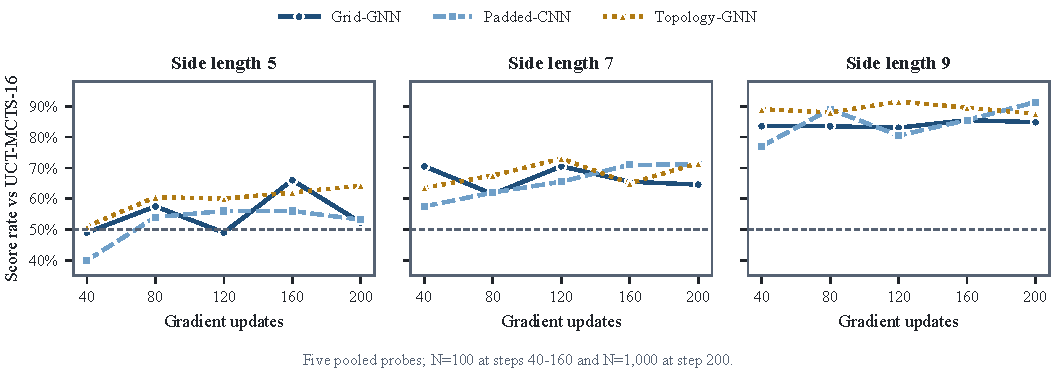
\includegraphics[width=0.96\linewidth]{fig2_checkpoint_curves.pdf}
  \caption{\raggedright Frozen pooled score-rate probes against UCT-MCTS-16 from
  \texttt{arena\_learning\_curve.csv}, retained only as a schedule and
  reconciliation visualization. The vertical scale is focused on 0.35--0.98.
  Steps 40--160 pool 100 game records per point, whereas step 200 pools 1,000;
  the receipt-bound audit reports the corresponding five-seed medians, ranges,
  and pair-score distributions. The probes support neither uncertainty,
  continuous-convergence, nor relative sample-efficiency inference.}
  \label{fig:checkpoint-curves}
\end{figure}

\begin{figure}[H]
  \centering
  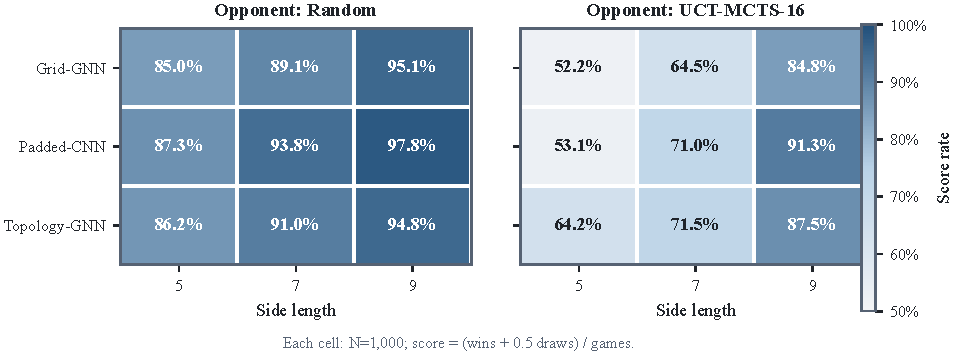
\includegraphics[width=0.92\linewidth]{fig3_model_size_opponent_heatmap.pdf}
  \caption{Pooled reconciliation heatmap from
  \texttt{final\_vs\_search.csv}; each cell aggregates 1,000 game records from
  five training-seed receipts. Table~\ref{tab:final-search} gives the primary
  five-seed median and range. Score is $(W+0.5D)/N$, not raw win rate. Colors
  do not encode uncertainty, multiplicity-adjusted significance, or unseen-size
  generalization.}
  \label{fig:final-heatmap}
\end{figure}

\subsection{Representation round robin}

Direct play exhibits heterogeneous seed-level outcomes
(Table~\ref{tab:round-robin}). Only Topology-GNN versus Grid-GNN at side length
7 has a seed-score median of 1.00; the other eight model-pair--size medians are
0.50, with wide ranges. No global ordering is supported.

\begin{table}[H]
  \centering
  \footnotesize
  \caption{\raggedright Seed-level score summaries from A's perspective in
  \texttt{representation\_round\_robin.csv}. Each cell is median [min, max]
  across five training-seed tasks. Every 200-game task contains two
  deterministic color-conditioned outcomes, each repeated 100 times; ranges
  are descriptive and no global ranking is inferred.}
  \label{tab:round-robin}
  \begin{tabular}{@{}lccc@{}}
    \toprule
    A vs.\ B & $n=5$ & $n=7$ & $n=9$ \\
    \midrule
    Topology-GNN vs.\ Grid-GNN & .50 [.50,1.00] & 1.00 [.50,1.00] & .50 [.50,1.00] \\
    Padded-CNN vs.\ Grid-GNN & .50 [.00,1.00] & .50 [.00,1.00] & .50 [.00,.50] \\
    Padded-CNN vs.\ Topology-GNN & .50 [.00,1.00] & .50 [.00,.50] & .50 [.00,1.00] \\
    \bottomrule
  \end{tabular}
\end{table}

Across all 9,000 round-robin games, each 200-game task contains exactly two
unique color-conditioned trajectories. Each aggregate therefore represents
five training seeds and ten unique trajectories, not 1,000 independent trials.

\subsection{Ablations}

\texttt{enforce} rejects repetitions, whereas \texttt{observe} admits them
while retaining history. In a 2,000-pair fixed-policy pilot at each of sizes 6
and 7, only two size-7 games triggered Superko and one trajectory diverged; all
winners agreed, no game truncated, and mean length changed by $-0.01017\%$.

All internal fixed gates for score ($\pm 5$ percentage points), relative length
($\pm 5\%$), and truncation passed for this policy, size set, and horizon. This
supports ``empirically similar under the sampled policy,'' not rule equivalence:
only one handcrafted policy was evaluated.

A preregistered five-seed extension covered six policies, two sizes, 120
matched pairs, and 240 replay-verified games. It observed no trigger or outcome
effect, but every practical-similarity gate failed: each cell had only ten
\texttt{observe} games, so $0/10$ has a 27.75\% Wilson upper bound, above the
1\% threshold. CycleSeeking's null result is a bounded search miss, and its
neural row is a one-game, one-update smoke checkpoint.

\subsection{Compute and reproducibility}

Runs used Python 3.10.20, PyTorch 2.7.1+cu118, deterministic CUDA 11.8, and an
RTX 4060 Laptop GPU. Mean per-seed training time was 489.8\,s for
\mbox{Padded-CNN}, 399.2\,s for \mbox{Grid-GNN}, and 440.0\,s for
\mbox{Topology-GNN} (1.85 aggregate training GPU-hours);
evaluation compute is not yet consolidated. One canonical manifest digest
(\texttt{1bbf2c9a9ecc...}) binds all 330 receipts. Independent aggregation
rechecked task identity, budgets, hashes, summaries, and all 30,600
task-indexed replay-verified game records;
for this completed D14--D16 bundle,
\texttt{formal\_ready=true} denotes artifact completeness, not superiority.

\section{Limitations and Broader Impact}
\label{sec:limitations}

\begin{itemize}
  \item The side-six paired-history witness is equal only under a mask-free
  Topology projection. Its implemented legal masks differ, so it is not an
  identical-observation-and-mask decision witness and does not establish a
  learned representation benefit.
  \item Results cover jointly trained sizes 5, 7, and 9, not zero-shot sizes 10
  or 12; history, logical-edge, cascade, and search-budget ablations remain.
  \item Grid-GNN and Topology-GNN differ in typed relations and hidden width, so
  their comparison mixes representation and architecture; the CNN adds a model
  family confound. Parameters and data are matched, but FLOPs, memory,
  transitions, and wall time are not.
  \item The primary replication count is five training seeds per cell. Each D16
  200-game seed-task contains only two unique color-conditioned trajectories,
  each repeated 100 times. Seed medians, ranges, and pair-score histograms are
  descriptive and provide no confidence interval or hypothesis test. A later
  preregistered diversified extension executed all planned games but failed its
  frozen trajectory-diversity gate and is therefore excluded here. A
  prospectively redesigned evaluation and independent verification remain
  required.
  \item \lifeline{} is one hand-designed game, so external validity to other
  games is untested; its Superko matrix is finite-policy evidence. The smoke
  neural condition and incomplete evaluation-compute accounting preclude
  broader efficiency claims.
\end{itemize}

\section{Conclusion}
\label{sec:conclusion}

\lifeline{} provides an auditable setting for separating rule state from the
learning interface in self-play. The side-five enumeration is a useful
negative control: latent logical-edge differences do not automatically imply
a legal-action, value, or optimal-action difference. The side-six witness
shows a complementary failure mode: a deliberately weakened, mask-free
projection can hide a history-dependent legality difference, even though the
implemented legal masks reveal it to the agent. Neither result establishes a
learned representation benefit.

The frozen baseline audit is intentionally modest. All 45 final seed scores
against Random exceed 0.5 on seen sizes, but UCT-MCTS-16 medians vary by model
and size, and duplicated trajectories rule out a global ranking. The resulting
resource is a benchmark and diagnostic protocol, not a claim that typed
logical edges or compact history are universally useful. The next empirical
step is a preregistered same-backbone factorial ablation with diversified
openings, independent verification, and explicitly held-out sizes; until that
evidence exists, stronger causal and cross-game conclusions remain open.

\subsection*{Reproducibility statement}
Sections~\ref{sec:protocol}--\ref{sec:experiments} and
Appendix~\ref{app:hyperparameters} specify the frozen protocol, model budgets,
statistics, and result boundaries. The accompanying claim ledger maps each
paper claim to compact aggregate CSV/JSON, append-only receipt-ledger JSONL,
and independent verifier outputs. Checkpoints, raw per-game logs, and local
task directories are not claimed as submission artifacts.

\bibliographystyle{plainnat}
\bibliography{references}

\appendix
\small

\section{Hyperparameters and Training Details}
\label{app:hyperparameters}

\begin{table}[H]
  \centering
  \small
  \caption{Frozen formal settings from
  \texttt{D14\_D16\_EXPERIMENT\_PROTOCOL.md}, shared by all three learned
  representations. They define the completed seen-size run, not an unseen-size
  or search-budget ablation.}
  \label{tab:hyperparameters}
  \begin{tabular}{ll}
    \toprule
    Setting & Value \\
    \midrule
    Training sizes / seeds & $\{5,7,9\}$ / 20260825--20260829 \\
    PUCT & 16 simulations, $c_{\mathrm{puct}}=1.5$ \\
    Root noise & $\alpha=0.3$, $\epsilon=0.25$ \\
    Temperature & 1.0 for 20 plies, then 0.1 \\
    Self-play / updates & 100 complete games / 200 gradient steps \\
    Replay / batch & 10,000 / 16 \\
    Optimizer & AdamW, lr $10^{-3}$, weight decay $10^{-4}$ \\
    Gradient clipping & global norm 5.0 \\
    Checkpoints & steps 40, 80, 120, 160, 200 \\
    Terminal rule & 256 plies; enforced Superko; no shaped reward \\
    Final evaluation & 200 games per seed and matchup \\
    Color control & 100 same-seed swapped-color pairs \\
    \bottomrule
  \end{tabular}
\end{table}

Targets are the masked root-visit distribution and the terminal result from the
stored player-to-act perspective. Absolute player payoffs are backed up through
the search tree because automatic skips can leave the same player to act after
a transition. Training loss is masked policy cross-entropy plus mean-squared
terminal value error.

\section{Additional Results and Reproducibility}
\label{app:reproducibility}

Canonical aggregates retain checkpoint, W/D/L, seed, loss, transition, and
timing fields. In the completed D14--D16 bundle, no formal task failed or
truncated; smoke runs and duplicate
views of the step-200 UCT matchup are excluded from the 30,600 task-indexed
replay-verified game records. The receipt-bound
\path{d14_d16_seed_pair_descriptive_audit.json} reconstructs all 330
receipts and 15,300 color-swapped pairs into 315 seed-task rows and 72 five-seed
summaries, matching all 72 canonical rows with zero mismatch. Its 45 D16 task
profiles each bind two color-conditioned trajectory hashes with 100 repetitions
apiece; all pair-score distributions remain descriptive. The paper's evidence
mapping names frozen
protocol/config hashes, compact aggregate CSV/JSON summaries, an append-only
JSONL receipt ledger, and independent verifier outputs. It does not claim that checkpoints, raw per-game logs, or
task directories are included in the submission artifacts.
Aggregation rejects missing or duplicate tasks, identity or budget drift,
truncation, color imbalance, and incomplete replay. Two interrupted runners
lack independent canonical files for their first two attempts, so no
per-attempt lineage is claimed.

\end{document}
